% v2-acmtog-sample.tex, dated March 7 2012
% This is a sample file for ACM Transactions on Graphics
%
% Compilation using 'acmtog.cls' - version 1.2 (March 2012), Aptara Inc.
% (c) 2010 Association for Computing Machinery (ACM)
%
% Questions/Suggestions/Feedback should be addressed to => "acmtexsupport@aptaracorp.com".
% Users can also go through the FAQs available on the journal's submission webpage.
%
% Steps to compile: latex, bibtex, latex latex
%
% For tracking purposes => this is v1.2 - March 2012
\documentclass{sig-alternate} % v 2.5

% --- Author Metadata here ---
\conferenceinfo{Sample Conferenve}{'15 Potsdam, Germany}
%\CopyrightYear{2007} % Allows default copyright year (20XX) to be over-ridden - IF NEED BE.
%\crdata{0-12345-67-8/90/01}  % Allows default copyright data (0-89791-88-6/97/05) to be over-ridden - IF NEED BE.
% --- End of Author Metadata ---

\begin{document}

\title{Project Light}

\numberofauthors{5}

\author{
\alignauthor
Cornelius Bock
%
\alignauthor
Daniel Werner
%
\alignauthor
Felix Wolff
%
\and
\texttt{\{cornelius.bock|daniel.werner|felix.wolff\}@student.hpi.de} \\ \\
\and
\alignauthor
Christoph Meinel\\
    \affaddr{\textit{Supervisior}}
%
\alignauthor
Konrad-Felix Krentz\\
    \affaddr{\textit{Supervisior}}
}

\maketitle

\begin{abstract}
Lorem ipsum dolor sit amet, consectetur adipisicing elit, sed do eiusmod
tempor incididunt ut labore et dolore magna aliqua. Ut enim ad minim veniam,
quis nostrud exercitation ullamco laboris nisi ut aliquip ex ea commodo
consequat. Duis aute irure dolor in reprehenderit in voluptate velit esse
cillum dolore eu fugiat nulla pariatur. Excepteur sint occaecat cupidatat non
proident, sunt in culpa qui officia deserunt mollit anim id est laborum.
\end{abstract}

\category{K.6.5}{Management Of Computing And Information Systems}{Security}

\terms{Internet of Things, Security}

\keywords{awesome, keywords, go, here}

\section{Introduction}
\label{sec:introduction}

\begin{itemize}
	\item short introduction internet of things
	\item some words about contiki
	\item current security and key distribution situation (akes)
	\item idea of transmitting keying material using light and phone app, why light, alternative solutions
	\item setup (android device/app, mote with light sensor)
\end{itemize}


\section{Related Work}
\label{sec:related_work}

\begin{itemize}
	\item LiDSN: A Method to Deploy Wireless Sensor Networks Securely based on light communication
	\item ...
\end{itemize}


\section{Communication Protocol}
\label{sec:communication_protocol}

In the following section, we describe the phases of the protocol. 
Each phase contains the necessary steps for the Android device and the mote.
Insights into the concrete implementation will be given in the Section~\ref{sec:implementation}.

\subsection{Calibration}
\label{sub:calibration}

The goal of the calibration phase is to establish light values for \textit{bright} and \textit{dark} on the mote.
By doing this in the beginning of the protocol, we can adapt to different lighting situations in the room and different brightness levels of the phone.

The task of the phone in this protocol stage is simple. 
It periodically sends \textit{bright} and \textit{dark} values, each with a certain period length $T$.
Simply said, it is blinking.

The mote on the other side measures $n$ light values using its light sensor.
The time between two measurements will probably not be equal to $T$, because the period length is unknown the mote at this point.
As long as \textit{bright} and \textit{dark} values are part of the $n$ measurements, the concrete time does not matter.
After reading $n$ values, the mote calculates reasonable numeric values for \textit{bright} and \textit{dark}.
For instance, this can be achieved by applying a \mbox{\textit{2-means}} algorithm (add reference to implementation).
After that, the mote is able to classify new light values.
In other words, it can read bits.

\subsection{Synchronization}
\label{sub:synchronization}

During synchronization, the mote learns the period length $T$.
This is necessary to be able to read light values at the right time (see Figure~\ref{fig:read_a_bit}).

In this phase, the phone just keeps sending \textit{bright} and \textit{dark} values with the period length $T$.
This is the same as during calibration.

The mote on the other hand now measures light values as fast as it can and classifies them as \textit{0} and \textit{1}.
Once it notices that the bit flips, it records the time when the switch happened.
After recording $m$ bit flips, it can calculate the average period length.

With completion of the first two phases, the mote is now able to read data sent by the phone.
It learned a decision threshold for decoding the bits and the period length to read values at the right time.
Figure~\ref{fig:read_a_bit} shows how data can be read. 
However, the concrete implementation slightly differs from that figure, see (add reference to implementation).

\begin{figure}
	\centering
	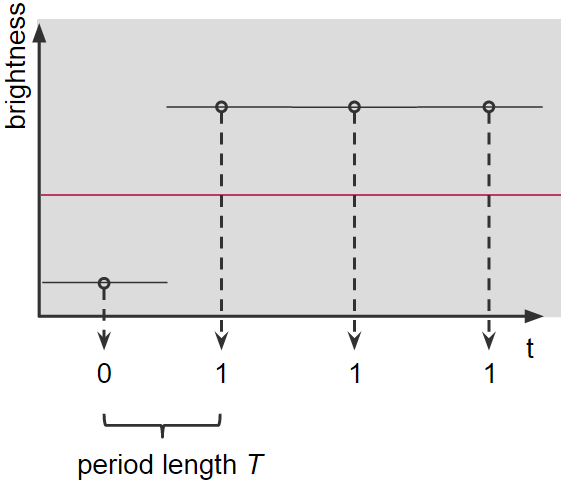
\includegraphics[scale=.5]{images/reading_data.png}
	\caption{Reading data: The black horizontal lines show the brightness emitted by the phone, the red line is the decision threshold for classifying \textit{0} and \textit{1}. Each arrow shows a point in time where the mote reads the value of the light sensor. The result here is the bit string 0111.}
	\label{fig:read_a_bit}
\end{figure}

\subsection{Initialization}
\label{sub:initialization}

\subsection{Data sending}
\label{sub:data_sending}

\subsection{Validation}
\label{sub:validation}



\section{Implementation}
\label{sec:implementation}

\begin{itemize}
	\item hamming code, crc32 checksum, when to read a bit (at the end of the period)
	\item Android app - functionality, flashlight, limitations
	\item contiki process - functionality, rtimer?, kmeans?, limitations
	\item driver wrapper to delay link layer initialization until key is initialized
\end{itemize}



\section{Results and Discussion}
\label{sec:results_and_discussion}

\begin{itemize}
	\item measure and evaluate maximum transmission speed, error rate
	\item is hamming code necessary (worth the doubled length) or CRC alone sufficient
	\item does the transmission rate have to be variable?
	\item "keep the phone busy" (wake up more often to prevent cpu from sleeping)
\end{itemize}



\section{Conclusion and Future Work}
\label{sec:future_work}

\begin{itemize}
	\item bidirectional communication using the LEDs of the mote (and maybe camera)
	\item 802.15.4 dongle to verify transmission (and do further initialization)
	\item initialize several mote together, separate synchronization and data sending
\end{itemize}

% Bibliography
\bibliographystyle{ACM-Reference-Format-Journals}
\bibliography{paper}

\end{document}
